%------------------------------------------------
\section{Cơ sở lý thuyết \& tổng quan}

%------------------------------------------------
\begin{frame}
\label{Maths}
	\frametitle{TỔNG QUAN TẤM PIN NĂNG LƯỢNG MẶT TRỜI}
	\begin{center}
		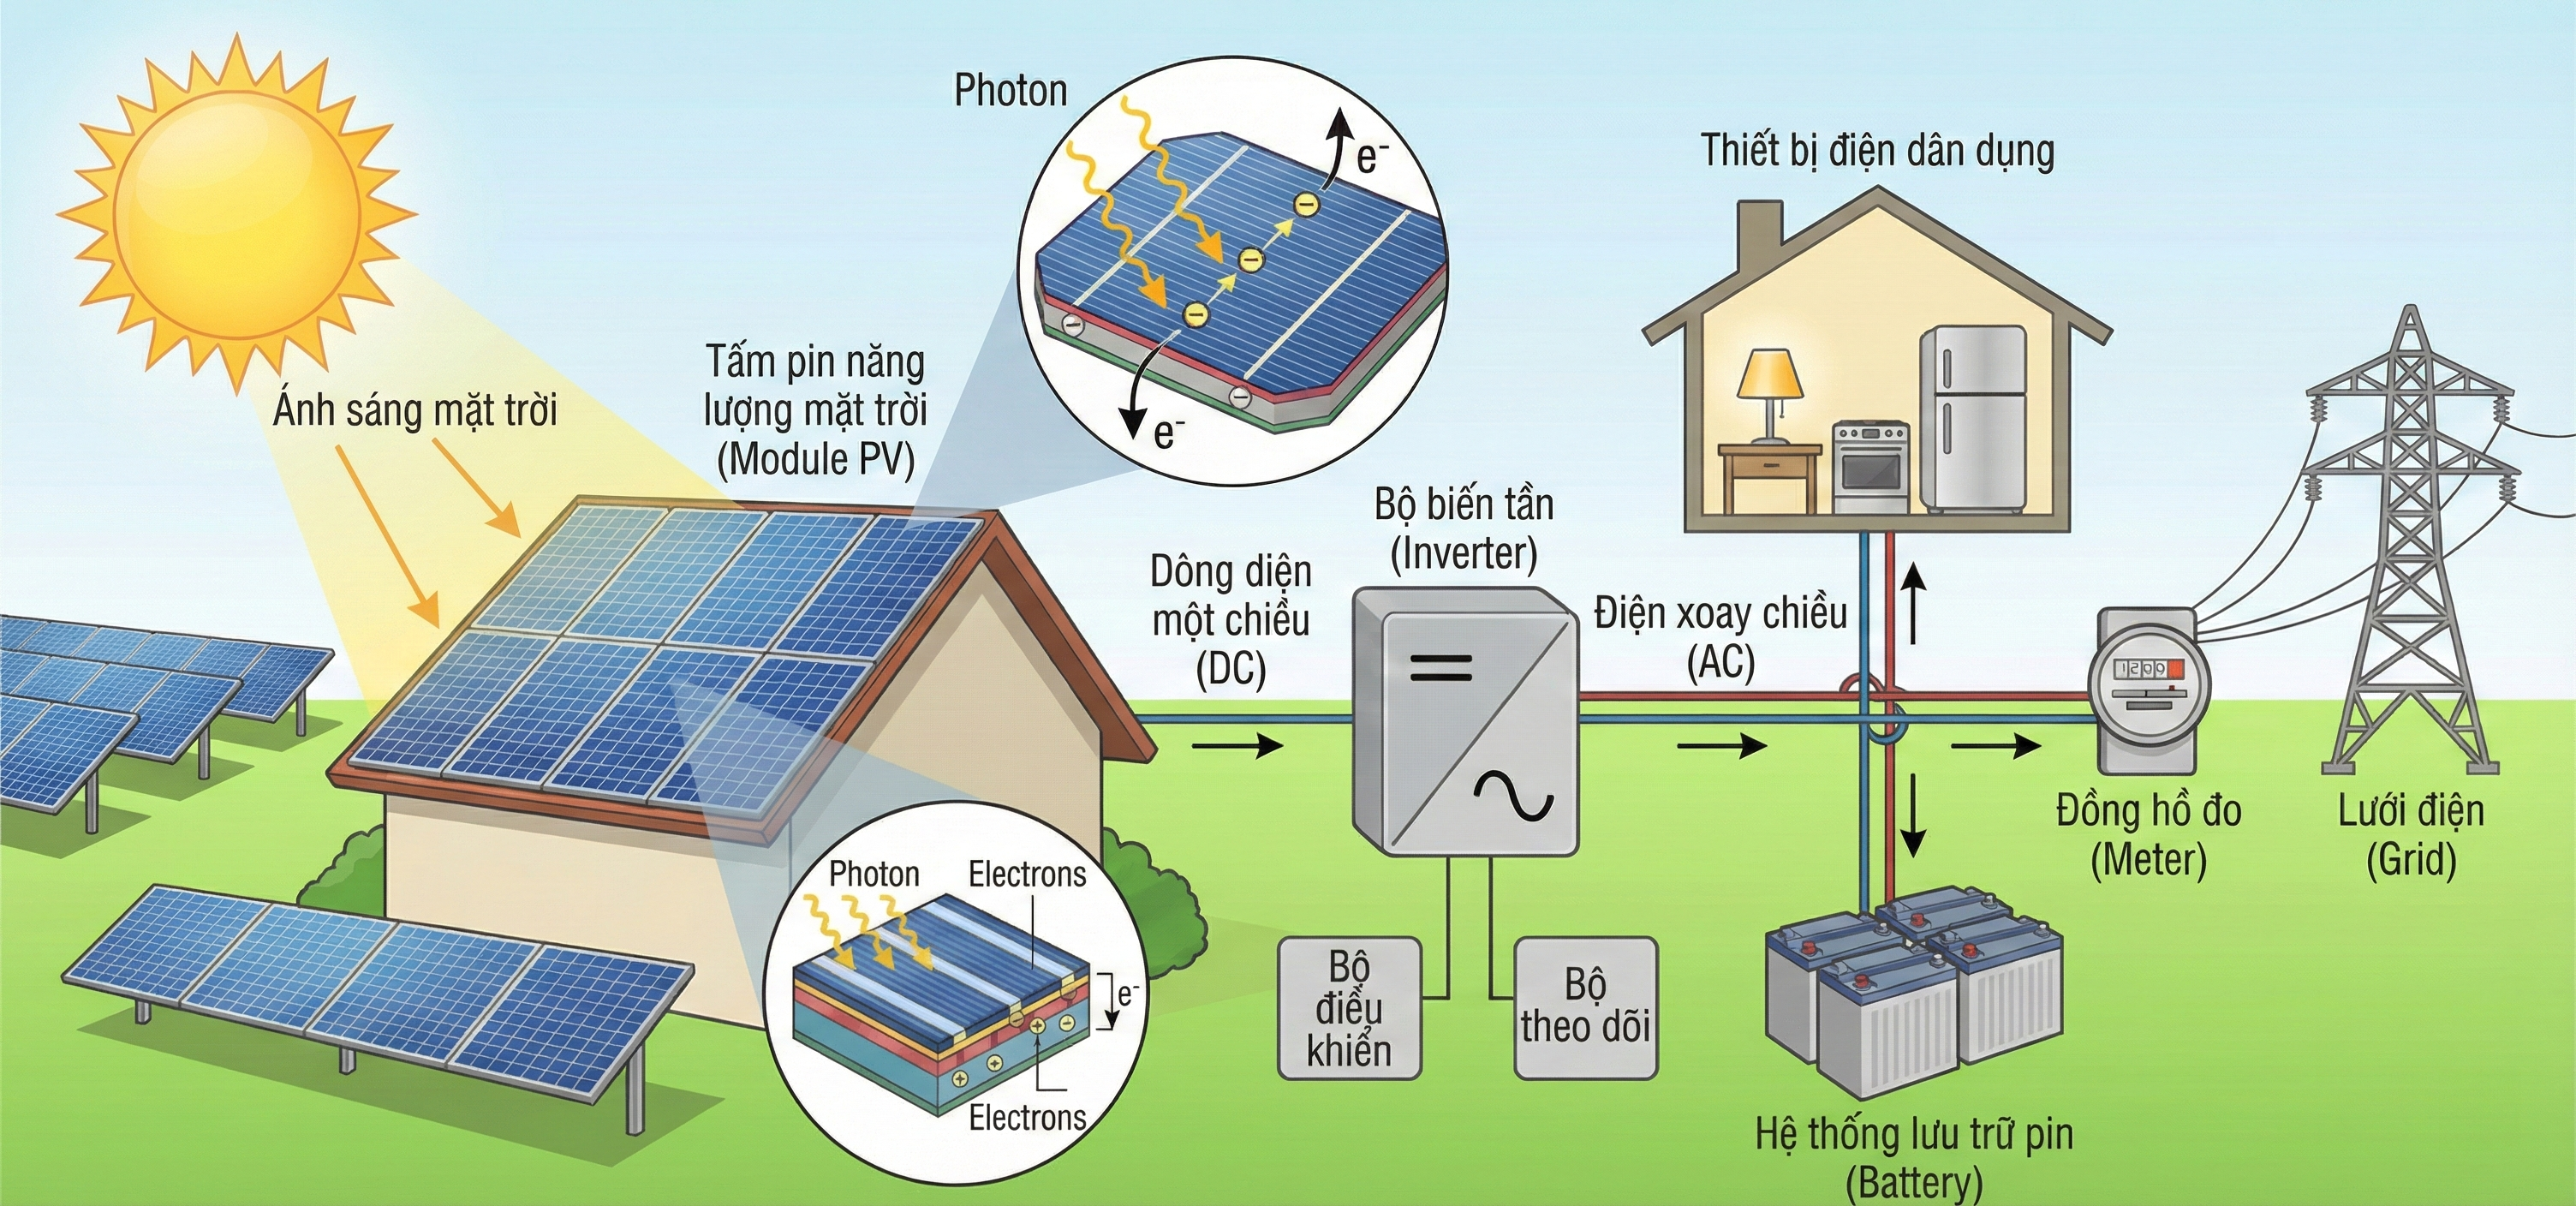
\includegraphics[width=0.8\textwidth]{images/TongQuan/pinmattroi.png}
	\end{center}
\end{frame}

%------------------------------------------------
\begin{frame}
	\frametitle{TÌNH HÌNH HỆ THỐNG PIN MẶT TRỜI TRÊN THẾ GIỚI}
	
	\vspace{0.3cm}
	
	\begin{columns}[t]
		% Cột 1: BÙNG NỔ
		\begin{column}{0.3\textwidth}
			\centering
			\includegraphics[width=0.5\textwidth]{images/TongQuan/icons/bungno.png}
			
			\vspace{0.3cm}
			
			{\Large\textbf{BÙNG NỔ}}
			
			\vspace{0.4cm}
			
			\small
			Diện mặt trời chiếm \\
			\textcolor{orange}{\textbf{73\%}} tổng công suất \\
			năng lượng tái tạo \\
			tăng thêm toàn cầu \\
			năm 2023.
		\end{column}

		\vrule width 1pt
		
		% Cột 2: CHI PHÍ
		\begin{column}{0.3\textwidth}
			\centering
			\includegraphics[width=0.5\textwidth]{images/TongQuan/icons/chiphi.png}
			
			\vspace{0.3cm}
			
			{\Large\textbf{CHI PHÍ}}
			
			\vspace{0.4cm}
			
			\small
			Chi phí lắp đặt đã giảm sâu \\
			\textcolor{orange}{\textbf{85\%}} sau một thập kỷ, trở \\
			thành nguồn năng lượng \\
			dễ tiếp cận nhất.
		\end{column}

		\vrule width 1pt
		
		% Cột 3: TIỀM NĂNG
		\begin{column}{0.3\textwidth}
			\centering
			\includegraphics[width=0.5\textwidth]{images/TongQuan/icons/tiemnang.png}
			
			\vspace{0.3cm}
			
			{\Large\textbf{TIỀM NĂNG}}
			
			\vspace{0.4cm}
			
			\small
			Việt Nam nằm trong \\
			``vùng đỏ'' bức xạ nhiệt, \\
			mang hữu tiềm năng tự \\
			nhiên lý tưởng để phát \\
			triển điện mặt trời.
		\end{column}
	\end{columns}
	
\end{frame}

\begin{frame}
\label{Bungno}
	\frametitle{TÌNH HÌNH HỆ THỐNG PIN MẶT TRỜI TRÊN THẾ GIỚI}
	\begin{center}
		\includegraphics[width=0.7\textwidth]{images/TongQuan/bieudobungno.png}
	\end{center}
\end{frame}

\begin{frame}
\label{Chiphi}
	\frametitle{TÌNH HÌNH HỆ THỐNG PIN MẶT TRỜI TRÊN THẾ GIỚI}
	\begin{center}
		\includegraphics[width=0.6\textwidth]{images/TongQuan/bieudochiphi.png}
	\end{center}
\end{frame}

\begin{frame}
\label{Nhiet}
	\frametitle{TÌNH HÌNH HỆ THỐNG PIN MẶT TRỜI TRÊN THẾ GIỚI}
	\begin{center}
		\includegraphics[width=0.8\textwidth]{images/TongQuan/bieudonhiet.png}
	\end{center}
\end{frame}

\begin{frame}
    \frametitle{TÌNH HÌNH HỆ THỐNG PIN MẶT TRỜI TRÊN VIỆT NAM}
    
    % [FIX 1] Giảm khoảng cách dưới tiêu đề (0.2 -> 0.1)
    \vspace{0.1cm} 
    
    \begin{columns}[T] 
        
        % --- CỘT TRÁI: BẢN ĐỒ ---
        \begin{column}{0.32\textwidth}
            \centering
            \vspace{0pt} 
            \includegraphics[width=0.95\textwidth]{images/TongQuan/bandonhietVietNam.png}
        \end{column}
        
        % --- CỘT PHẢI: NỘI DUNG ---
        \begin{column}{0.65\textwidth}
            \vspace{0pt} 
            
            % === PHẦN 1: PHÁP LÝ ===
            % [FIX 2] Giảm kích thước khung chứa icon (1.2cm -> 0.9cm)
            \begin{minipage}[c]{0.9cm}
                % [FIX 3] Giảm size icon (1.0cm -> 0.75cm) cho gọn
                \includegraphics[width=0.75cm]{images/TongQuan/icons/phaply.png}
            \end{minipage}%
            \hspace{0.1cm}%
            \begin{minipage}[c]{8.8cm} 
                {\Large\textbf{\textcolor{blue!70!black}{PHÁP LÝ}}}
            \end{minipage}
            
            % [FIX 4] Giảm khoảng cách dưới tiêu đề mục (0.1 -> 0.05)
            \vspace{0.05cm}
            
            \footnotesize
            \begin{itemize}
                % [FIX 5] Giảm khoảng cách giữa các item (0.1 -> 0.02)
                \setlength\itemsep{0.02cm} 
                \item Chuyển từ giai đoạn chính sách giá ưu đãi (kích cầu đầu tư ồ ạt) sang giai đoạn phát triển bền vững và có kiểm soát.
                \item Tập trung kiểm soát an toàn lưới điện và đặc biệt ưu tiên khuyến khích mô hình điện mặt trời \textbf{tự sản tự tiêu} (thay vì bán lên lưới).
            \end{itemize}
            
            % [FIX 6] Giảm khoảng cách lớn giữa 2 phần (0.4 -> 0.25)
            \vspace{0.25cm} 
            
            % === PHẦN 2: TIỀM NĂNG ===
            \begin{minipage}[c]{0.9cm}
                \includegraphics[width=0.75cm]{images/TongQuan/icons/tiemnangVietNam.png}
            \end{minipage}%
            \hspace{0.1cm}%
            \begin{minipage}[c]{8.8cm}
                {\Large\textbf{\textcolor{orange}{TIỀM NĂNG}}}
            \end{minipage}
            
            \vspace{0.05cm}
            
            \footnotesize
            \begin{itemize}
                \setlength\itemsep{0.02cm}
                \item \textbf{Việt Nam} nằm trong nhóm quốc gia có bức xạ mặt trời \textbf{tốt nhất Đông Nam Á}, đặc biệt tại miền Trung và Nam Bộ (bức xạ $>$4.6 kWh/kWp/ngày; $>$2500 giờ nắng/năm).
                \item \textbf{Miền Nam} phù hợp phát triển cả trang trại lớn và điện áp mái; \textbf{Miền Bắc} tuy bức xạ thấp hơn nhưng vẫn hiệu quả cho mô hình áp mái kết hợp lưu trữ.
            \end{itemize}
            
        \end{column}
    \end{columns}
\end{frame}

% Định nghĩa màu nền xanh
\definecolor{CardBlue}{HTML}{B1CDFC}

\begin{frame}[shrink=5]
    \frametitle{TÌNH HÌNH HỆ THỐNG PIN MẶT TRỜI TẠI VIỆT NAM}
    
    % Giảm khoảng cách dưới tiêu đề để tiết kiệm không gian
    \vspace{-0.3cm}
    
    \begin{columns}[t, onlytextwidth] % onlytextwidth giúp căn lề chuẩn hơn
        
        % Thiết lập style chung cho các card để code gọn gàng
        \tcbset{
            mycardstyle/.style={
                colback=CardBlue,       % Yêu cầu 3: Full nền xanh
                colframe=CardBlue!80!black, % Viền đậm hơn chút cho đẹp (hoặc để CardBlue nếu muốn ẩn)
                arc=8pt,                % Bo góc box
                boxrule=0pt,            % Bỏ viền dày
                left=2pt, right=2pt, top=2pt, bottom=2pt, % Tối ưu lề (Yêu cầu 1: giảm overfull)
                equal height group=A,   % Yêu cầu 4: Ép 3 cột cao bằng nhau
                fontupper=\tiny,        % Set font chữ nhỏ toàn bộ
                halign=center,          % Căn giữa nội dung
                valign=top              % Căn nội dung từ trên xuống
            }
        }

        % --- Card 1 ---
        \begin{column}{0.32\textwidth}
            \begin{tcolorbox}[mycardstyle]
                % Icon + Tiêu đề
                \includegraphics[height=0.8cm]{images/TongQuan/icons/dienmattroiquymolon.png}
                \par\vspace{0.1cm}
                {\scriptsize\textbf{ĐIỆN MẶT TRỜI\\QUY MÔ LỚN}}
                
                \vspace{0.1cm}
                % Nội dung (căn trái)
                \begin{flushleft}
                    \textbullet\ Nguồn cung cấp sản lượng điện lớn đóng góp vào lưới điện quốc gia.\\[0.1cm]
                    \textbullet\ Các dự án kỷ lục: nhà máy Dầu Tiếng, tổ hợp Trung Nam.
                \end{flushleft}
                
                \vfill % Đẩy ảnh xuống đáy (Yêu cầu 4)
                
                % Yêu cầu 2: Ảnh bo góc bằng TikZ Clip
                \begin{tikzpicture}
                    \clip [rounded corners=6pt] (0,0) rectangle (\linewidth, 1.8cm); 
                    \node[anchor=south west, inner sep=0] at (0,0) {\includegraphics[width=\linewidth, height=1.8cm]{images/TongQuan/trungnam.jpg}};
                \end{tikzpicture}
            \end{tcolorbox}
        \end{column}

        % --- Card 2 ---
        \begin{column}{0.32\textwidth}
            \begin{tcolorbox}[mycardstyle]
                \includegraphics[height=0.8cm]{images/TongQuan/icons/dienmattroiapmai.png}
                \par\vspace{0.1cm}
                {\scriptsize\textbf{ĐIỆN MẶT TRỜI\\ÁP MÁI}}
                
                \vspace{0.1cm}
                \begin{flushleft}
                    \textbullet\ Tận dụng mái nhà xưởng và hộ gia đình.\\[0.1cm]
                    \textbullet\ Ưu tiên hàng đầu: không tốn đất, giảm tải tại chỗ cho lưới điện.
                \end{flushleft}
                
                \vfill
                
				\vspace{0.3cm}
                \begin{tikzpicture}
                    \clip [rounded corners=6pt] (0,0) rectangle (\linewidth, 1.8cm);
                    \node[anchor=south west, inner sep=0] at (0,0) {\includegraphics[width=\linewidth, height=1.8cm]{images/TongQuan/apmai.png}};
                \end{tikzpicture}
            \end{tcolorbox}
        \end{column}

        % --- Card 3 ---
        \begin{column}{0.32\textwidth}
            \begin{tcolorbox}[mycardstyle]
                \includegraphics[height=0.8cm]{images/TongQuan/icons/dienmattroidoclap.png}
                \par\vspace{0.1cm}
                {\scriptsize\textbf{ĐIỆN MẶT TRỜI\\ĐỘC LẬP}}
                
                \vspace{0.1cm}
                \begin{flushleft}
                    \textbullet\ Khu vực chưa có điện lưới hoặc công trình độc lập.\\[0.1cm]
                    \textbullet\ Cần tính toán kỹ pin lưu trữ để đảm bảo ổn định.
                \end{flushleft}
                
                \vfill
                
                \begin{tikzpicture}
                    \clip [rounded corners=6pt] (0,0) rectangle (\linewidth, 1.8cm);
                    \node[anchor=south west, inner sep=0] at (0,0) {\includegraphics[width=\linewidth, height=1.8cm]{images/TongQuan/doclap.png}};
                \end{tikzpicture}
            \end{tcolorbox}
        \end{column}
        
    \end{columns}
    
    \vspace{0.1cm}
    \centering
    \fcolorbox{black!10}{white}{
    \parbox{0.95\textwidth}{
        \tiny \textbf{Tổng kết:} Sự cộng hưởng giữa tiềm năng bức xạ dồi dào và hành lang pháp lý khuyến khích tự sản tự tiêu tạo nền tảng vững chắc để Việt Nam phát triển năng lượng mặt trời hiệu quả và bền vững.
    }}
\end{frame}

% Định nghĩa màu sắc giống trong ảnh
\definecolor{mypaleblue}{RGB}{189, 215, 238} % Màu xanh nhạt cho đường kẻ
\definecolor{myorange}{RGB}{197, 90, 17}    % Màu cam đậm cho tiêu đề (nếu cần)
\definecolor{myblueicon}{RGB}{0, 112, 192}  % Màu xanh cho icon

% --- KHAI BÁO LỆNH BO GÓC BẰNG TIKZ (ĐẶT NGOÀI FRAME) ---
% Nguyên lý: Vẽ 1 ảnh tàng hình để lấy kích thước -> Tạo khung cắt bo tròn -> Vẽ ảnh thật đè lên
\newcommand{\roundimg}[2]{ % Tham số: #1 = chiều cao, #2 = đường dẫn ảnh
    \begin{tikzpicture}[baseline=(img.center)]
        \node[inner sep=0pt, opacity=0] (measure) {\includegraphics[height=#1]{#2}}; % Ảnh tàng hình đo size
        \clip[rounded corners=8pt] (measure.south west) rectangle (measure.north east); % Cắt bo góc
        \node[inner sep=0pt] (img) at (measure.center) {\includegraphics[height=#1]{#2}}; % Ảnh thật
    \end{tikzpicture}
}
% -----------------------------------------------------------------------

\begin{frame}
    \frametitle{CÁC DẠNG HƯ HỎNG PHỔ BIẾN}

    \vspace*{-0.5cm} 
    
    \begin{columns}[T]
        
        % --- CỘT 1 ---
        \begin{column}{0.32\textwidth}
            \begin{minipage}[c]{0.18\textwidth}
                \includegraphics[width=\linewidth]{images/TongQuan/icons/quanghoc.png} 
            \end{minipage}%
            \hspace{0.1cm}
            \begin{minipage}[c]{0.80\textwidth}
                \textbf{\footnotesize Suy Thoái Quang Học}
            \end{minipage}
            
            \vspace{0.1cm}
            \scriptsize \raggedright
            \begin{itemize}
                \setlength\itemsep{0.05cm}
                \setlength\parskip{0pt}
                \item \textbf{\textcolor{orange}{Bụi bẩn:}} Giảm khả năng hấp thụ ánh sáng.
                \item \textbf{\textcolor{orange}{Ố màu:}} Lão hóa vật liệu.
                \item \textbf{\textcolor{orange}{Bong tróc:}} Tách lớp kính bảo vệ.
            \end{itemize}
            
            \vspace{0.05cm}
            \centering
            % SỬ DỤNG LỆNH TIKZ ĐÃ TẠO Ở TRÊN
            \roundimg{1.6cm}{images/TongQuan/suythoaiquanghoc.png}
        \end{column}

        % --- KẺ DỌC 1 ---
        \begin{column}{0.02\textwidth}
            \centering
            \raisebox{-0.8cm}{\color{mypaleblue}\rule{1pt}{4.0cm}}
        \end{column}

        % --- CỘT 2 ---
        \begin{column}{0.32\textwidth}
            \begin{minipage}[c]{0.18\textwidth}
                \includegraphics[width=\linewidth]{images/TongQuan/icons/matketnoidien.png}
            \end{minipage}%
            \hspace{0.1cm}
            \begin{minipage}[c]{0.80\textwidth}
                \textbf{\footnotesize Mất Kết Nối Điện}
            \end{minipage}
            
            \vspace{0.1cm}
            \scriptsize \raggedright
            \begin{itemize}
                \setlength\itemsep{0.05cm}
                \setlength\parskip{0pt}
                \item \textbf{\textcolor{orange}{Vết nứt:}} Do tác động cơ học/nhiệt.
                \item \textbf{\textcolor{orange}{Điểm nóng:}} Gây quá nhiệt cục bộ.
                \item \textbf{\textcolor{orange}{Ngắn mạch:}} Hư hỏng cell pin.
            \end{itemize}
            
            \vspace{0.05cm}
            \centering
            % SỬ DỤNG LỆNH TIKZ
            \roundimg{1.6cm}{images/TongQuan/matketnoidien.jpg}
        \end{column}

        % --- KẺ DỌC 2 ---
        \begin{column}{0.02\textwidth}
            \centering
            \raisebox{-0.8cm}{\color{mypaleblue}\rule{1pt}{4.0cm}}
        \end{column}

        % --- CỘT 3 ---
        \begin{column}{0.32\textwidth}
            \begin{minipage}[c]{0.18\textwidth}
                \includegraphics[width=\linewidth]{images/TongQuan/icons/phancung.png}
            \end{minipage}%
            \hspace{0.1cm}
            \begin{minipage}[c]{0.80\textwidth}
                \textbf{\footnotesize Hư Hỏng Phần Cứng}
            \end{minipage}
            
            \vspace{0.1cm}
            \scriptsize \raggedright
            \begin{itemize}
                \setlength\itemsep{0.05cm}
                \setlength\parskip{0pt}
                \item \textbf{\textcolor{orange}{PID:}} Suy giảm do điện thế cảm ứng.
                \item \textbf{\textcolor{orange}{Diode hỏng:}} Mất chức năng bypass.
                \item \textbf{\textcolor{orange}{Lỗi dây:}} Ăn mòn, đứt gãy.
            \end{itemize}
            
            \vspace{0.05cm}
            \centering
            % SỬ DỤNG LỆNH TIKZ
            \roundimg{1.6cm}{images/TongQuan/huhongphancung.png}
        \end{column}
    \end{columns}
    
    % --- FOOTER ---
    \vspace{0.2cm}
    \centering
    \tiny 
    \parbox{0.95\textwidth}{
        Xuất phát từ đặc thù 'có thể nhìn thấy', đề tài tập trung nghiên cứu Nhận diện Suy thoái quang học và sẽ phân tích chi tiết các dạng lỗi này ở phần tiếp theo.
        
        \vspace{0.1cm}
        \textbf{Tổng kết Chương 1:} Từ cơ sở thực tiễn về tiềm năng và thiệt hại do hư hỏng tấm pin đã nêu, Chương 2 sẽ đi sâu phân tích các phương pháp kiểm tra và giám sát nhằm giải quyết vấn đề này.
    }
\end{frame}

\begin{frame}
\label{Cachuhong}
	\frametitle{CÁC DẠNG HƯ HỎNG PHỔ BIẾN}
	\begin{center}
		\includegraphics[width=0.6\textwidth]{images/TongQuan/cachuhong.png}
	\end{center}
\end{frame}

%------------------------------------------------
\section{Phương pháp đề xuất}

\begin{frame}
    \frametitle{GIỚI THIỆU VỀ UAV}

    % --- 1. KÉO SÁT LÊN TRÊN ---
    \vspace{-0.3cm}

    % --- 2. DANH SÁCH ---
    \footnotesize
    \begin{itemize}
        \setlength\itemsep{0pt}
        \setlength\parskip{0pt}
        \item Nhóm chọn giải pháp kiểm tra hệ thống bằng thiết bị bay không người lái (UAV) tích hợp Camera quang học (RGB).
        \item Hướng tiếp cận này khắc phục nhược điểm về chi phí cao và tốn kém nhân lực của các phương pháp truyền thống.
        \item Giải pháp loại bỏ tình trạng quá tải, tốn thời gian và nguy cơ bỏ sót lỗi khi phân tích thủ công lượng lớn hình ảnh.
    \end{itemize}

    \vspace{0.2cm} % Tăng khoảng cách một chút để thoáng hơn

    % --- PHẦN NỘI DUNG CHÍNH ---
    \begin{columns}[T, onlytextwidth]
        % --- CỘT TRÁI: BẢNG ĐÁNH GIÁ ---
        % Giảm độ rộng cột trái một chút để nhường chỗ cho cột phải
        \begin{column}{0.45\textwidth}
            \centering % <--- THÊM LỆNH NÀY ĐỂ CANH GIỮA BẢNG TRONG CỘT (DỊCH PHẢI 1 TÍ)
            \begin{table}[h]
                \scriptsize
                \renewcommand{\arraystretch}{1.2} % Tăng nhẹ giãn dòng cho dễ đọc
                \setlength{\tabcolsep}{3pt}
                % Sử dụng tỷ lệ phần trăm để bảng tự co giãn tốt hơn
                \begin{tabular}{|p{0.25\linewidth}|p{0.68\linewidth}|}
                    \hline
                    \rowcolor{blue!70}\textcolor{white}{\textbf{Đánh giá}} & \cellcolor{blue!70} \\
                    \hline
                    \cellcolor{green!20}\textbf{Ưu điểm} & Tối ưu chi phí, tốc độ; giảm tải nhân lực, dễ triển khai. \\
                    \hline
                    \cellcolor{red!20}\textbf{Hạn chế} & Chỉ phát hiện lỗi bề mặt; độ chính xác phụ thuộc đk bay. \\
                    \hline
                \end{tabular}
            \end{table}
        \end{column}

        % --- CỘT PHẢI: SƠ ĐỒ QUY TRÌNH MỚI ---
        % Tăng độ rộng cột phải để chứa sơ đồ lớn hơn
        \begin{column}{0.53\textwidth}
            \centering
            % Sử dụng resizebox để ép toàn bộ sơ đồ vừa khít chiều ngang cột
            \resizebox{1\linewidth}{!}{%
                \begin{tikzpicture}[
                    % Định nghĩa kiểu cho các hộp và nhãn
                    boxstyle/.style={
                        draw,
                        rectangle,
                        fill=blue!15, % Màu nền xanh nhạt giống ảnh
                        align=center,
                        font=\bfseries\small, % Chữ in đậm, to vừa
                        text width=3.2cm, % Độ rộng cố định cho các hộp
                        minimum height=1.2cm,
                        inner sep=5pt
                    },
                    labelstyle/.style={
                        align=center,
                        font=\scriptsize, % Chữ chú thích nhỏ hơn
                        text width=3.2cm,
                        below=0.2cm % Khoảng cách nằm dưới hộp
                    },
                    arrowstyle/.style={->, >=latex, thick} % Kiểu mũi tên
                ]

                    % 1. Node Drone ở trên cùng, giữa
                    % Thay đường dẫn ảnh bằng ảnh thực tế của bạn: images/PhuongPhap/drone.png
                    \node (drone) at (0, 3) {\includegraphics[width=2.5cm, keepaspectratio]{images/PhuongPhap/drone.png}};

                    % 2. Các hộp quy trình chính (Đặt hộp số 2 ở giữa tâm 0,0)
                    \node [boxstyle] (step2) at (0,0) {2. Thu thập dữ liệu RGB};
                    % Hộp 1 nằm bên trái hộp 2
                    \node [boxstyle, left=0.6cm of step2] (step1) {1. Lập kế hoạch bay};
                    % Hộp 3 nằm bên phải hộp 2
                    \node [boxstyle, right=0.6cm of step2] (step3) {3. AI Detect (Deep Learning)};

                    % 3. Các nhãn chú thích bên dưới các hộp
                    \node [labelstyle] at (step1.south) {Thiết lập đường bay tự động};
                    \node [labelstyle] at (step2.south) {Chụp ảnh, gắn thẻ GPS, ghép bản đồ};
                    \node [labelstyle] at (step3.south) {Phân tích lỗi \& Định vị tọa độ};

                    % 4. Các mũi tên kết nối
                    % Mũi tên nét đứt từ Drone xuống hộp 2
                    \draw [arrowstyle, dashed, very thick, gray!80] (drone.south) -- (step2.north);
                    % Mũi tên từ 1 sang 2
                    \draw [arrowstyle] (step1) -- (step2);
                    % Mũi tên từ 2 sang 3
                    \draw [arrowstyle] (step2) -- (step3);

                \end{tikzpicture}
            }% Kết thúc resizebox
        \end{column}
    \end{columns}
\end{frame}

\begin{frame}
\label{UAV}
	\frametitle{GIỚI THIỆU VỀ UAV}
	\begin{center}
		\includegraphics[width=0.6\textwidth]{images/PhuongPhap/UAV.png}
	\end{center}
\end{frame}

% --- ĐỊNH NGHĨA MÀU ---
\definecolor{customBlueTitle}{HTML}{6FA8DC}
\definecolor{customBlueBody}{HTML}{CFE2F3}
\definecolor{customGreenTitle}{HTML}{70AD47}
\definecolor{customGreenBody}{HTML}{B6D7A8}
\definecolor{customGreenCardBG}{HTML}{D9EAD3}

% --- ĐƯỜNG DẪN ẢNH ---
\newcommand{\pathIcons}{C:/Users/minhk/Downloads/SolarPanelSlideLatex/images/PhuongPhap/icons/}
\newcommand{\pathImages}{C:/Users/minhk/Downloads/SolarPanelSlideLatex/images/PhuongPhap/}

% --- MACRO VẼ THẺ TIKZ ---
\newcommand{\drawCustomCard}[2]{%
    \begin{tikzpicture}
        \def\cardW{3.45cm}%
        \def\totalH{2.15cm}% Giữ kích thước nhỏ gọn
        \def\splitY{1.2cm}%
        \def\rad{0.2cm}%
        \def\imgH{0.95cm}%

        % --- PHẦN 1: ẢNH ---
        \begin{scope}
            \clip [rounded corners=\rad] (0,\splitY) -- (\cardW,\splitY) -- (\cardW,\totalH) -- (0,\totalH) -- cycle;
            \node[anchor=south west, inner sep=0] at (0,\splitY) {
                \includegraphics[width=\cardW, height=\imgH, keepaspectratio=false]{#1}
            };
        \end{scope}

        % --- PHẦN 2: TEXT ---
        \begin{scope}
            \path[fill=customGreenCardBG, rounded corners=\rad] (0,0) -- (\cardW,0) -- (\cardW,\splitY) -- (0,\splitY) -- cycle;
            \node[anchor=center] at (\cardW/2, \splitY/2) {
                \begin{minipage}{3.25cm}
                    \centering
                    \fontsize{5}{6}\selectfont 
                    \color{black} 
                    #2
                \end{minipage}
            };
        \end{scope}
    \end{tikzpicture}%
}

\begin{frame}[t]
    % Giữ nguyên vị trí bắt đầu
    \vspace{-0.4cm} 
    \frametitle{KIỂM TRA MẮT THƯỜNG \& PHƯƠNG PHÁP BỔ TRỢ}

    % --- CẤP ĐỘ 1 ---
    {
        \setbeamercolor{block title}{bg=customBlueTitle, fg=white}
        \setbeamercolor{block body}{bg=customBlueBody, fg=black}
        \setbeamertemplate{blocks}[rounded][shadow=false]

        \begin{block}{\centering \raisebox{-0.5ex}{\includegraphics[height=1.2em, keepaspectratio]{\pathIcons search.png}} \enspace \textbf{CẤP ĐỘ 1: KIỂM TRA BẰNG MẮT THƯỜNG}}
            \vspace{-0.1cm}
            \begin{columns}
                \column{0.75\textwidth}
                \fontsize{6}{7}\selectfont 
                \begin{itemize}
                    \setlength\itemsep{0pt}
                    \setlength\parskip{0pt}
                    \setlength\leftmargini{0.4cm}
                    \item Bước sàng lọc đầu tiên phát hiện lỗi bề mặt (kính, frame...).
                    \item Quan sát trực tiếp vật mẫu dưới điều kiện ánh sáng mạnh.
                    \item Ưu điểm: Tốc độ xử lý nhanh, chi phí thấp, dễ thực hiện.
                    \item Nhược điểm: Phụ thuộc chủ quan và thị lực người kiểm tra.
                    \item Hạn chế: Không thấy được lỗi ẩn sâu (micro-crack).
                \end{itemize}

                \column{0.21\textwidth}
                \centering
                \begin{tikzpicture}
                    \begin{scope}
                        \clip [rounded corners=0.2cm] (0,0) rectangle (2.5cm, 0.85cm);
                        \node[anchor=south west, inner sep=0] at (0,0) {
                            \includegraphics[width=2.5cm, height=0.85cm, keepaspectratio=false]{\pathImages visual_inspection_worker.png}
                        };
                    \end{scope}
                \end{tikzpicture}
            \end{columns}
            \vspace{-0.1cm}
        \end{block}
    }

    % --- MŨI TÊN (ĐIỀU CHỈNH KHOẢNG CÁCH ĐỂ ĐẨY CẤP 2 XUỐNG) ---
    \begin{center}
        \vspace{-0.3cm} % [Fix] Nới lỏng khoảng cách trên mũi tên (-0.5 -> -0.3)
        
\begin{tikzpicture}[scale=1]
            \fill[fill=customBlueBody, draw=none] (-0.2,0.3) -- (0.2,0.3) -- (0.2,0) -- (0.4,0) -- (0,-0.4) -- (-0.4,0) -- (-0.2,0) -- cycle;
        \end{tikzpicture}
        \vspace{-0.1cm} % [Fix] Nới lỏng khoảng cách dưới mũi tên (-0.5 -> -0.1) -> Đẩy Cấp 2 xuống
    \end{center}



	\vspace{-0.3cm}
    % --- CẤP ĐỘ 2 ---
    \begin{tcolorbox}[
        enhanced,
        colframe=customGreenTitle,
        colbacktitle=customGreenTitle,
        coltitle=white,
        colback=customGreenBody,
        fonttitle=\bfseries\small,
        title={CẤP ĐỘ 2: CÁC PHƯƠNG PHÁP BỔ TRỢ CHUYÊN SÂU},
        arc=1.5mm, boxrule=0.5pt,
        left=1pt, right=1pt, top=0pt, bottom=0pt, 
        toptitle=1pt, bottomtitle=0pt,
        halign title=center
    ]
        \begin{columns}[t, onlytextwidth]
            % --- CỘT 1 ---
            \column{0.33\textwidth}
            \centering
            \begin{minipage}{3.4cm}
                \centering
                % [Fix] Dùng raisebox -2pt để hạ Icon xuống ngang hàng với chữ
                \raisebox{-2pt}{\includegraphics[height=0.8em]{\pathIcons electricity_icon.png}}
                \enspace \tiny \textbf{\textcolor{black}{ĐIỆN HỌC}} 
            \end{minipage}
            \vspace{0.05cm} 
            \drawCustomCard{\pathImages iv_curve_device.png}{%
                Đo đường cong I-V kiểm tra sức khỏe dòng điện và hiệu suất thực tế.%
            }

            % --- CỘT 2 ---
            \column{0.33\textwidth}
            \centering
            \begin{minipage}{3.4cm}
                \centering
                % [Fix] Căn thẳng hàng
                \raisebox{-2pt}{\includegraphics[height=0.7em]{\pathIcons camera_icon.png}}
                \enspace \tiny \textbf{\textcolor{black}{HÌNH ẢNH}}
            \end{minipage}
            \vspace{0.05cm}
            \drawCustomCard{\pathImages el_images.png}{%
                \begin{itemize}
                    \setlength\itemsep{0pt}
                    \setlength\leftmargini{0.2cm}
                    \item[•] EL: Nhìn xuyên thấu vết nứt.
                    \item[•] UV-F: Đánh giá lão hóa.
                \end{itemize}%
            }

            % --- CỘT 3 ---
            \column{0.33\textwidth}
            \centering
            \begin{minipage}{3.4cm}
                \centering
                % [Fix] Căn thẳng hàng
                \raisebox{-2pt}{\includegraphics[height=0.8em]{\pathIcons flask_icon.png}}
                \enspace \tiny \textbf{\textcolor{black}{PHÂN TÍCH VẬT LIỆU}}
            \end{minipage}
            \vspace{0.05cm}
            \drawCustomCard{\pathImages spectrometer_lab.png}{%
                Máy Quang phổ phân tích chuyên sâu cấu trúc vật liệu trong Lab.%
            }
        \end{columns}
    \end{tcolorbox}

    % --- FOOTER (ĐẨY XUỐNG THÊM) ---
	\vspace{-0.1cm}
    \centering
    \tiny \textit{`\textbf{Khám lâm sàng}' $\to$ `\textbf{Xét nghiệm y khoa}' để kết luận chính xác}
\end{frame}

\begin{frame}
	\frametitle{TỔNG HỢP \& SO SÁNH CÁC PHƯƠNG PHÁP}

\end{frame}

